\subsection{双向链表}

\begin{frame}\ft{\subsecname}
\begin{dingyi}[双向链表]
每个结点有两个指针域:
\begin{itemize}
\item[$\diamond$]
一个指向其直接前趋的指针域{\tt prior}
\item[$\diamond$]
一个指向其直接后继的指针域{\tt next}
\end{itemize}
这样形成的链表有两个不同方向的链,故称为双向链表。
\end{dingyi}
\end{frame}

\begin{frame}\ft{\subsecname}
\begin{itemize}
\item 
和单链表类似,双向链表一般也增设一个头结点,能使双向链表上的某些运算变得方便。\\
\item
将头结点和尾结点链接起来,可形成循环链表,称为“双向循环链表”。\\
\item
双向链表是为了克服单链表单向性的缺陷而引入的。\\
\end{itemize}•
\end{frame}
%
\begin{frame}[fragile]\ft{\subsecname}

\textcolor{acolor5}{双向链表结点的类型定义:}
\begin{lstlisting}[language=C,basicstyle=\ttfamily]
typedef struct DuLNode
{
  ElemType data;
  struct DuLNode * prior, * next;
}DuLNode;
\end{lstlisting}

\begin{figure}
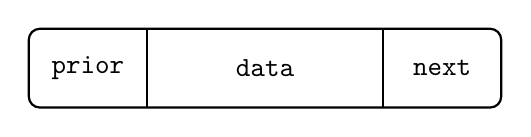
\begin{tikzpicture}
\def\x{1.5}
\def\y{1}
\def\r{0}
\draw[thick,rounded corners] (0,0)rectangle(4*\x,\y);
\draw[thick,thick] (\x,0)--(\x,\y);
\draw[thick,thick] (3*\x,0)--(3*\x,\y);
\node[]at(0.5*\x,0.5*\y){\tt prior};
\node[]at(2*\x,0.5*\y){\tt data};
\node[]at(3.5*\x,0.5*\y){\tt next};
\end{tikzpicture}
\caption{双向链表的结点示意图}
\end{figure}•
\end{frame}
%
%
%
\begin{frame}[fragile]\ft{\subsecname}
\begin{figure}
\centering
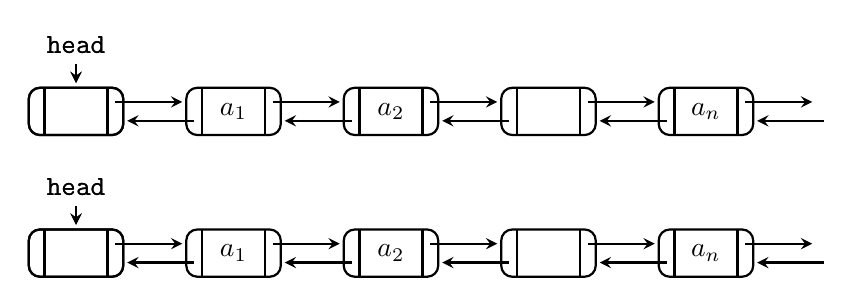
\begin{tikzpicture}[scale=1]
\def \x{1}
\def \y{0.6}

\foreach \c in {0,3}{
\ifthenelse{ 0 = \c}{
\foreach \r in {0,2,4,6,8}{
\ifthenelse{  6 = \r }{
\node[left] at (\r*\x+\x,\c*\y+0.5*\y) {$\cd$};
}{
\draw[thick,rounded corners] (\r*\x+0.0*\x,\c*\y+0)rectangle(\r*\x+1.2*\x,\c*\y+\y);
\draw[thick,thick] (\r*\x+0.2*\x,\c*\y+0) -- (\r*\x+0.2*\x,\c*\y+\y);
\draw[thick,thick] (\r*\x+1.0*\x,\c*\y+0) -- (\r*\x+1.0*\x,\c*\y+\y);
}
\ifthenelse{ 8 = \r}{
}{
\draw[thick,<-,>=stealth] 
(\r*\x+1.25*\x,\c*\y+0.3*\y)--(\r*\x+2.10*\x,\c*\y+0.3*\y);
\draw[thick,->,>=stealth] 
(\r*\x+1.10*\x,\c*\y+0.7*\y)--(\r*\x+1.95*\x,\c*\y+0.7*\y);
}
}

\node[]at(2.6,\c*\y+0.5*\y){$a_1$};
\node[]at(4.6,\c*\y+0.5*\y){$a_2$}; 
\node[]at(8.6,\c*\y+0.5*\y){$a_n$};
\draw[thick,->,>=stealth] (0.6,\c*\y+1.5*\y)node[above] {\tt head} --(0.6,\c*\y+1.1*\y);
}{
\foreach \r in {0}{
\draw[thick,rounded corners] (\r*\x+0.0*\x,\c*\y+0)rectangle(\r*\x+1.2*\x,\c*\y+\y);
\draw[thick,thick] (\r*\x+0.2*\x,\c*\y+0) -- (\r*\x+0.2*\x,\c*\y+\y);
\draw[thick,thick] (\r*\x+1.0*\x,\c*\y+0) -- (\r*\x+1.0*\x,\c*\y+\y);

%\filldraw[fill=black!20,fill opacity=0.5](\r*\x+0.0*\x,\c*\y+0)rectangle(\r*\x+0.2*\x,\c*\y+\y);  
%\filldraw[fill=red!20,fill opacity=0.5](\r*\x+0.2*\x,\c*\y+0)rectangle(\r*\x+1.0*\x,\c*\y+\y); 
%\filldraw[fill=black!20,fill opacity=0.5](\r*\x+1.0*\x,\c*\y+0)rectangle(\r*\x+1.2*\x,\c*\y+\y); 
\draw[thick,->,>=stealth] (0.6,\c*\y+1.5*\y)node[above] {\tt head} --(0.6,\c*\y+1.1*\y);
}
}
}

\end{tikzpicture}
\caption{带头结点的双向链表形式}
\end{figure}

\end{frame}
%
\begin{frame}[fragile]\ft{\subsecname}
双向链表结构具有对称性,设{\tt p}指向双向链表中的某一个结点,则其对称性可描述为:
\begin{lstlisting}[basicstyle=\ttfamily]
(p->prior)->next == p == (p->next)->prior;
\end{lstlisting}
\end{frame}
%
%
\begin{frame}\ft{双向链表的基本操作:插入}
将值为$e$的结点插入双向链表中,插入前后链表的变化如图:

\begin{figure}
\centering
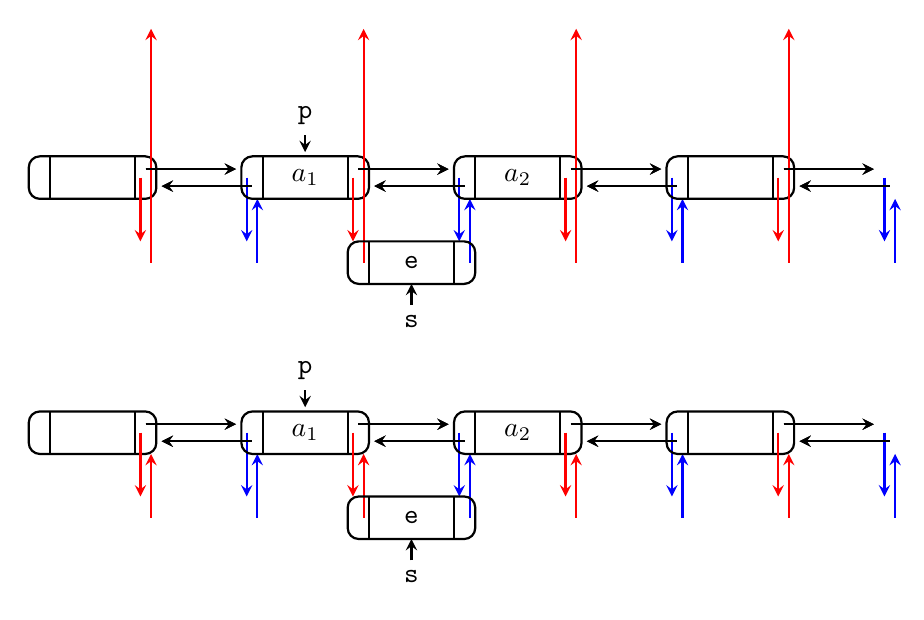
\begin{tikzpicture}[scale=0.9]
\def \x{1.5}
\def \y{0.6}

\foreach \c in {0,6}
{
\foreach \r in {0,2,4,6}
{
\ifthenelse{  0 = \r \OR 6 = \r}
{
\node[left] at (\r*\x+\x,\c*\y+0.5*\y) {$\cd$};
}
{
\draw[thick,rounded corners] (\r*\x+0.0*\x,\c*\y+0)rectangle(\r*\x+1.2*\x,\c*\y+\y);
\draw[thick,thick] (\r*\x+0.2*\x,\c*\y+0) -- (\r*\x+0.2*\x,\c*\y+\y);
\draw[thick,thick] (\r*\x+1.0*\x,\c*\y+0) -- (\r*\x+1.0*\x,\c*\y+\y);
}

\ifthenelse{ 6 = \r \OR 2 = \r}
{
\ifthenelse{ 2 = \r \AND \c = 6}
{
\draw[thick,<-,>=stealth] (\r*\x+1.25*\x,\c*\y+0.3*\y)--(\r*\x+2.10*\x,\c*\y+0.3*\y);
\draw[thick,->,>=stealth] (\r*\x+1.10*\x,\c*\y+0.7*\y)--(\r*\x+1.95*\x,\c*\y+0.7*\y);
}
{}

\ifthenelse{ 2 = \r \AND \c = 0}
{
\draw[thick,->,>=stealth,red] (\r*\x+1.05*\x,\c*\y+0.5*\y)--(\r*\x+1.05*\x,\c*\y-\y);
\draw[thick,<-,>=stealth,red] (\r*\x+1.15*\x,\c)--(\r*\x+1.15*\x,\c*\y-1.5*\y);

\draw[thick,->,>=stealth,blue] (\r*\x+2.05*\x,\c*\y+0.5*\y)--(\r*\x+2.05*\x,\c*\y-\y);
\draw[thick,<-,>=stealth,blue] (\r*\x+2.15*\x,\c*\y)--(\r*\x+2.15*\x,\c*\y-1.5*\y);
}{}

}{
\draw[thick,<-,>=stealth] (\r*\x+1.25*\x,\c*\y+0.3*\y)--(\r*\x+2.1*\x,\c*\y+0.3*\y);
\draw[thick,->,>=stealth] (\r*\x+1.1*\x,\c*\y+0.7*\y)--(\r*\x+1.95*\x,\c*\y+0.7*\y);
}
}

\node[]at(2.6*\x,\c*\y+0.5*\y){$a_1$};
\node[]at(4.6*\x,\c*\y+0.5*\y){$a_2$}; 
\draw[thick,->,>=stealth] (2.6*\x,\c*\y+1.5*\y)node[above] {\tt p} --(2.6*\x,\c*\y+1.1*\y);


\def\r{3}
\draw[thick,rounded corners] (\r*\x+0.0*\x,\c*\y-2*\y)rectangle(\r*\x+1.2*\x,\c*\y-\y);
\draw[thick,thick] (\r*\x+0.2*\x,\c*\y-2*\y) -- (\r*\x+0.2*\x,\c*\y-\y);
\draw[thick,thick] (\r*\x+1.0*\x,\c*\y-2*\y) -- (\r*\x+1.0*\x,\c*\y-\y);

\node[]at(\r*\x+0.6*\x,\c*\y-1.5*\y){\tt e}; 
\draw[thick,->,>=stealth] (\r*\x+0.6*\x,\c*\y-2.5*\y)node[below] {\tt s} --(\r*\x+0.6*\x,\c*\y-2*\y);

}

\end{tikzpicture}
%\caption{双向链表的插入}
\end{figure}

\end{frame}
%
%
\begin{frame}[fragile]\ft{双向链表的基本操作:插入}
1、若仅给出直接前驱{\tt p},则钩链时必须注意先后次序:“先右后左”。
\begin{lstlisting}[language=C,basicstyle=\ttfamily]
s = (DuLNode *) malloc(sizeof(DuLNode));
s->data = e;
s->next = p->next;
p->next->prior = s;
p->next = s;
s->prior = p;
\end{lstlisting}

\end{frame}


\begin{frame}[fragile]\ft{双向链表的基本操作:插入}
2、若同时给出直接前驱{\tt p}和直接后继{\tt q},则钩链时无需注意先后次序。
\begin{lstlisting}[language=C,basicstyle=\ttfamily]
s = (DuLNode *)malloc(sizeof(DuLNode));
s->data = e;
p->next = s; s->next = q;
s->prior = p; q->prior = s;
\end{lstlisting}
 

\end{frame}


\begin{frame}[fragile]\ft{双向链表的基本操作:删除}
设要删除的结点为{\tt p},删除时可以不引入新的辅助变量,可以直接先断链,再释放结点。
\begin{lstlisting}[language=C,basicstyle=\ttfamily]
p->prior->next = p->next;
p->next->prior = p->prior;
free(p);
\end{lstlisting}
\pause

\textcolor{acolor5}{注意:}
与单链表的插入和删除不同,在双向链表中插入和删除必须同时修改两个方向上指针域的指向。

\end{frame}